\documentclass[a4paper,11pt]{article}
%\documentclass[a4paper,9pt,landscape]{article}
\usepackage[english]{babel}
%\usepackage[utf8]{inputenc}
\usepackage{graphicx}
\usepackage{fullpage}
\usepackage{amsmath}
\usepackage{pdfpages}
\usepackage{listings}
\usepackage{color}
\usepackage{multicol}
\usepackage{fancyhdr}
\usepackage[top=1.5cm, bottom=4cm, left=2.5cm, right=2.5cm]{geometry}
\usepackage{hyperref}
\usepackage{verbatim}
\setlength{\voffset}{-9pt}
%\setlength{\hoffset}{-1in}
%\setlength{\marginparsep}{0.5cm}


\setlength{\parindent}{1cm}
%\setlength{\parskip}{-0.1cm}
%\setlength{\columnseprule}{0.4pt}
\setlength{\footskip}{0.5cm}
\setlength{\headheight}{15pt}
\setlength{\headsep}{2cm}

\fancypagestyle{tcr}{%
  \fancyhf{} %clear all headers and footers fields
  \fancyhead[R]{\thepage}
  \fancyhead[L]{\textbf{Lab No 4 TDDC78}}
  \renewcommand{\headrulewidth}{0.4pt}
}

\definecolor{dkgreen}{rgb}{0,0.6,0}
\definecolor{gray}{rgb}{0.5,0.5,0.5}
\definecolor{mauve}{rgb}{0.58,0,0.82}
\lstset{
  title=\lstname,
  frame=t,
  %aboveskip=-0.5cm, 
  %belowskip=0pt,
  basicstyle=\footnotesize\ttfamily,
  keywordstyle=\color{blue},          % keyword style
  commentstyle=\color{dkgreen},       % comment style
  stringstyle=\color{mauve},         % string literal style
  showstringspaces=false,         % underline spaces within strings
  tabsize=2,
  language=C,
  title=\caption,
  %xleftmargin=-1cm
}


\begin{document}
%% title stuff
\title{Lab No 4 TDDC78}
\author{Linus Mellberg (linme560) \and Oskar Aagaard (oskaa489)}
\date{\today}
\maketitle
\pagebreak
%\setcounter{page}{1}
%\begin{multicols}{2}
\thispagestyle{tcr}
\pagestyle{tcr}
%\tableofcontents

\section{Particle Simulation}
By simulating particle moving and interacting in a box the gas law $pV = nRT$ can be verified.
The problem is solved for the 2 dimensional case, where the particles are moving in a rectangular plane.
$p$ is the pressure, this is calculated by counting the momentum transferred to the box wall divided by the length of it every timestep.
$V$ is the area of the box (2d volume).
$n$ is the number of particles in the box.
$T$ is the temperature of the gas which is proportional to the average energy of the particles.
Energy is calculated as $\frac{v^2}{2}$ where v is the velocity of a particle.
The mass of the particles is the same for all of them and each particle weighs one mass unit.
$R$ is a constant.
The verification of the gas law is done by calculating this $R=\frac{pV}{nT}$ for different setups and verify that it is constant.

\subsection{Implementation}
A sequential program that implements this simulation need to do the following.
Distribute a $n$ particles and their velocities uniformly in the box.
Then for each timestep:
\begin{itemize}
  \item Check for collisions between particles, for every collision calculate new velocities and positions for the particles.
  \item For every non-colliding particle move it.
  \item For every particle that has moved outside the box move it inside and calculate the momentum transferred to the wall.
\end{itemize}
In this implementation each particle can only collide with one other particle during each timestep.
This is a simplification, but it is reasonable if the number of collisions is low.
This means that the number of particles has to be low compared to the area of the box.

The above algorithm gives an asymptotic complexity of $O(N^2)$ if $N$ is the number of particles.
The number of timesteps can be included here but is left out, this is assumed to be constant for the rest of the report.
The quadratic complexity can be improved by a simplification.
If the velocities of the particles are small, particles will only interact with other particles if they are close to each other at the beginning of each timestep.
The box can be divided into a number of regions and only particles that are in the same region at the start of each timestep needs to be checked for collisions.
Some collisions will be ignored if this is done, since there are no interactions between particles in different regions.
If the timestep and velocities are small this will not affect the final result much.
To minimize the number of missed collisions, the area of each region divided by its circumference, should be maximized.
A reasonably good way to do this is to divide the box into equally big rectangles.
The asymptotic complexity for this algorithm is $O(r(\frac{N}{r})^2) = O(\frac{N^2}{r})$ if $r$ is the number of regions that the box are divided into.
This algorithm is also much more suited for parallelization.

The way we implementeded it was to use one region for each process.
Each process gets a rectangular region, it then creates particles randomly in this region.
A timestep is run according to the algorithm above independently in each region.
When a timestep has finished, particles that has moved outside a process' region is sent to the process that handles the region it ended up in.
To move particles between processes an MPI datatype was created to represent a particle.
After each timestep a list of particles is sent to all neighbouring processes.
Particles are only sent to neighbours that are adjacent horizontally and vertically.
If a particle should move diagonally between regions it will end up in one of the adjacent regions instead and then moved to the correct region after the next timestep.
This should not occur often and will probably not affect the result much.
Only particles that moves between regions are communicated with MPI.
This means that the interprocess communication is fairly low.
Internally each process uses linked lists to store particles.
This implementation should have the asymptotic complexity $O((\frac{N}{p})^2)$ where $p$ is the number of processes.

\subsection{Results}
The results of particle simulation seems to agree with the gas law.
The program was executed with some different parameters and R was calculated for each run.
The generated data can be seen in table \ref{data}.
R seems to be constant.

In figure \ref{exec} the execution times for different problemsizes and number of ranks can be seen.
It is hard to tell how fast these graphs grows, it is at least faster than linear.
To check if the complexity $O((\frac{N}{p})^2)$ seems correct.
Each datapoint is divided by the complexity that corresponds to that point.
This will result in some sort of corrected excecution time which has the unit $sp^2N^{-2}$ where $s$ is seconds, $p$ is ranks and $N$ is number of particles.
If the assumption about the complexity is correct all datapoints should now be the same.
The plot can be seen in figure \ref{corr}.
The curves in the plot seems to converge to a constant of about $5 \cdot 10^{-5}$.
For low problem sizes the more ranks seem to create more overhead, but if the problem size grows this overhead doesn't make a big difference.
Especially the run with 32 ranks is a lot slower than the others, and no run is slower than 1 second.
This run needs two nodes and the extra second here is probably due to initialization of these.

If the problem size is large enough it seems like one should be able to calulate the expected execution time of our program with the formula $T = 5 \cdot 10^{-5} \frac{N^2}{p^2}$


\begin{table}[h!]
  \begin{center}
  \caption{Data from particle simulation.}
  \label{data}
  \begin{tabular}[h]{|l|l|l|l|l|}
    \hline
    T       & n     & V (dimensions)         & p          & R\\
    \hline
    418.41  & 20000 & 1.00e+08 (10000x10000) & 8.3256e-2  & 0.99 \\ 
    415.40  & 20000 & 8.40e+07 (28000x3000)  & 9.8715e-2  & 1.00 \\ 
    411.55  & 9984  & 1.00e+08 (10000x100000)& 4.0979e-2  & 1.00 \\ 
    2521.34 & 9984  & 1.00e+08 (10000x10000) & 0.249838   & 0.99 \\
    912.35  & 23744 & 5.91e+09 (85832x68832) & 3.657e-3   & 1.00 \\
    \hline
  \end{tabular}
  \end{center}
\end{table}

\begin{figure}[!h]
  \caption{Execution times.}
  \label{exec}
  \includegraphics[scale=0.9]{../plots/exec_time.png}
\end{figure}

\begin{figure}[!h]
  \caption{Corrected execution times.}
  \label{corr}
  \includegraphics[scale=0.9]{../plots/corr_time.png}
\end{figure}

\clearpage

\begin{comment}
%bulletlist
\paragraph\noindent\textbf{Overview of the linear program}
\begin{itemize}
\renewcommand{\labelitemi}{$\bullet$}
\item Load image from disk
\item Calculate average RGB sum
\item Calculate output image
\item Write image to disk
\end{itemize}

%picture import
\begin{figure}[!h]
  \caption{Run times related to number of cores for the different images.}
  \label{runtime_vs_cores}
  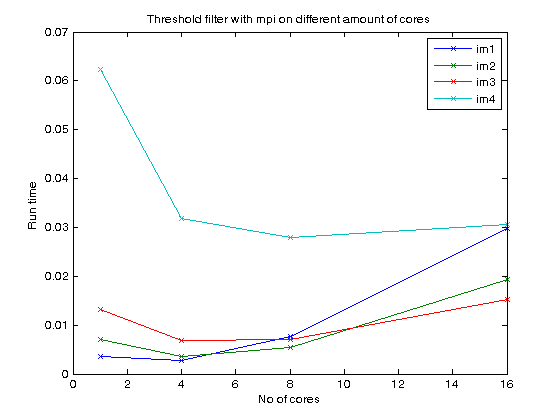
\includegraphics[scale=0.9]{../plots/runtimevscoresthres.png}
\end{figure}

%table
\begin{table}[h!]
  \caption{$MPixels/Second$ when running with different amount of threads and on different data.}
  \label{mpixelspersecond}
  \begin{tabular}[h]{|l|l|l|l|l|l|}
    \hline
                      & 1      & 2      & 4      & 8      & 16\\
    \hline
    im1.ppm           & 135.41 & 183.31 & 184.94 & 68.89  & 21.77\\ 
    im2.ppm           & 150.01 & 209.17 & 274.71 & 201.65 & 63.15\\ 
    im3.ppm           & 146.25 & 209.72 & 274.44 & 275.62 & 138.23\\ 
    im4.ppm           & 145.07 & 212.56 & 286.41 & 332.90 & 297.42\\
    \hline
  \end{tabular}
\end{table}

%citation from bibliography
\cite{fenwick}

%bibliography
\clearpage
\begin{thebibliography}{9}
  \bibitem{fenwick}
    Binary Indexed Trees,
    \emph{Algortihmist}.\\
    \url{http://community.topcoder.com/tc?module=Static\&d1=tutorials\&d2=binaryIndexedTrees}
  \bibitem{ppm}
    Mark Nelson,
    \emph{Arithmetic Coding + Statistical Modeling = Data Compression}, 1991.\\
    \url{http://marknelson.us/1991/02/01/arithmetic-coding-statistical-modeling-data-compression/}
  \bibitem{ppmc}
    PPM
    \url{http://www.cs.ucf.edu/courses/cap5015/ppm.pdf}

\end{thebibliography}a

%sourcecode listing
\lstinputlisting[caption=mpiblur.c]{../mpiblur.c}
\end{comment}

\clearpage
\section{Source code}
Files that are included but not listed here were downloaded from the course webpage and not modified.

\lstinputlisting[caption=simulate.c]{../simulate.c}
\clearpage
\lstinputlisting[caption=structures.h]{../structures.h}
\clearpage
\lstinputlisting[caption=structures.c]{../structures.c}
\clearpage
\lstinputlisting[caption=definitions.h]{../definitions.h}
\clearpage
\end{document}
